\documentclass[a4paper, norsk, 12pt]{extarticle}
\usepackage[T1]{fontenc} % Vise norske tegn
\usepackage[latin1]{inputenc} % For � kunne skrive norske tegn
\usepackage{babel} % Tilpasning til norsk
\usepackage{graphicx} % For � inkludere grafikk
\usepackage{amsmath,amssymb} % Ekstra matematikkfunksjoner
\usepackage{titlesec}

% Juster sidemarginer
\usepackage[margin=.9in, includefoot]{geometry}

% \usepackage{adjustbox}
% \usepackage{tabularx}
% \usepackage{relsize}
% \usepackage{booktabs}

% Topptekst
\usepackage{fancyhdr}
\pagestyle{fancy}
\fancyhead[L]{Oblig1b - 2017}
\fancyhead[C]{MAT121}
\fancyhead[R]{Magnus �ian}
\usepackage{pdfpages}


% Redefinerer "\section" til "Oppgave n"
% Nummerering skjer automatisk
\titleformat{\section}{\center \normalfont \Large \bfseries}
{Oppgave\ \thesection}{2.3ex plus .2ex}{}
\titlespacing{\subsection}{2em}{*1}{*5}

\begin{document}

%Oppgave 1
\section{}
\begin{itemize}

% 1)
\item[1)]
Vi har matrisen
\begin{align*}
	A = \begin{bmatrix}  5 & 2 & 0  \\  0 & 3 & 1  \\ 0 & 0 & 0  \end{bmatrix}
\end{align*}
og vektoren
\begin{align*}
	\bold{b} = \begin{bmatrix} 3 \\ 2 \\ 2 \end{bmatrix} .
\end{align*}
Den augmenterte matrisen $\begin{bmatrix} A & \bold{b} \end{bmatrix}$ er inkonsistent og f�lgelig er $\bold{b} \notin \text{Col} A$.

% 2)
\item[2)]
Eksempel p�  $4 \times 3$ matrise med rank($A$) $ = 1 $:
\begin{align*}
\begin{bmatrix} 2 & 3 & 4 \\ 0 & 0 & 0 \\ 0 & 0 & 0 \\ 0 & 0 & 0 \end{bmatrix}
\end{align*}

% 3)
\item[3)]
Vi har at $A^2 = I$ er inverterbar per definisjon inverterbar med $A^{-1} = A$. 

% 4)
\item[4)]
$A$ er en $5 \times 6$ matrise og da vil Col $A \in \mathbb{R}^5 \neq \mathbb{R}^3$. \\�
Vi har at dim Nul($A$) $ = \text{antall kolonner} - \text{rank($A$)} = 6 - 3 = 3$.

% 5)
\item[5)]
Vi har at  $\text{rank($A$)}  = \text{antall kolonner} - \text{dim Nul($A$)} = 5 - 2 = 3$.

% 6)
\item[6)]
Vektoren $\bold{x}$ er vist i figuren: \\ 
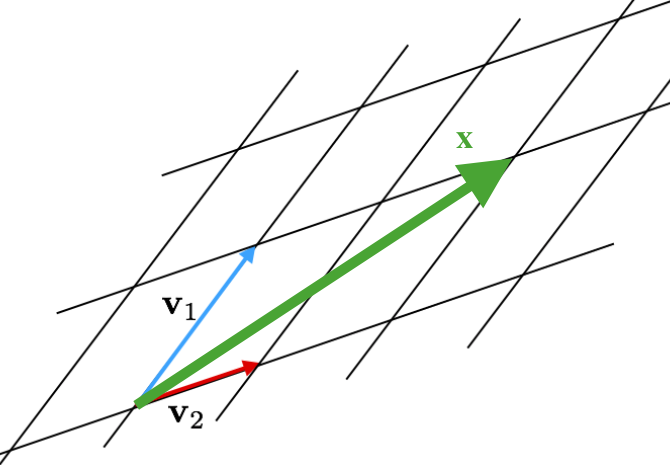
\includegraphics[width=10cm, height=6cm]{oppg_6}

% 7)
\item[7)]
Vi har at $[x]_{\mathcal{B}} = \begin{bmatrix} 2 \\ -1 \end{bmatrix}$.

% 8)
\pagebreak
\item[8)]
Utf�rer rekkeoperasjoner p� matrisen
\begin{align*}
	\begin{bmatrix} 1 & 2 & 3 & 1 & 0 & 0 \\  0 & 1 & 2 & 0 & 1 & 0  \\ 0 & 0 & 1 & 0 & 0 & 1  \end{bmatrix} 
\sim 	\begin{bmatrix}  1 & 0 & -1 & 1 & -2 & 0 \\ 0 & 1 & 2 & 0 & 1 & 0 \\ 0 & 0 & 1 & 0 & 0 & 1 \end{bmatrix}
\sim 	\begin{bmatrix}  1 & 0 & 0 & 1 & -2 & 1 \\ 0 & 1 & 0 & 0 & 1 & 0 \\ 0 & 0 & 1 & 0 & 0 & 1 \end{bmatrix}.
\end{align*}
Det gir at
\begin{align*}
A^{-1} = \begin{bmatrix} 1 & -2 & 1 \\ 0 & 1 & -2 \\ 0 & 0 & 1 \end{bmatrix}.
\end{align*}
\end{itemize}

% Oppgave 2
\section{}
Vi har at $(I-A) = I$ og $(I-A)^{-1} = I$. Det gir $(I-A)(I-A)^{-1} = I^2 = I$ og $(I-A)^{-1}(I-A) = I^2 = I$. 
Da f�lger det per definisjon av inverterbarhet at $(I-A)$ er inverterbar med $(I-A)^{-1} = I + A + A^2 + ... + A^{p-1}$.
\end{document}
